\documentclass{beamer}
\usepackage[utf8]{inputenc}

\usetheme{Madrid}
\usecolortheme{default}
\usepackage{amsmath,amssymb,amsfonts,amsthm}
\usepackage{txfonts}
\usepackage{tkz-euclide}
\usepackage{listings}
\usepackage{adjustbox}
\usepackage{array}
\usepackage{tabularx}
\usepackage{gvv}
\usepackage{lmodern}
\usepackage{circuitikz}
\usepackage{tikz}
\usepackage{graphicx}

\setbeamertemplate{page number in head/foot}[totalframumber]

\usepackage{tcolorbox}
\tcbuselibrary{minted,breakable,xparse,skins}

\definecolor{bg}{gray}{0.95}
\lstset{
    language=C,
    basicstyle=\ttfamily\small,
    keywordstyle=\color{blue},
    stringstyle=\color{orange},
    commentstyle=\color{green!60!black},
    numbers=left,
    numberstyle=\tiny\color{gray},
    breaklines=true,
    showstringspaces=false,
}

%------------------------------------------------------------
\title{9.4.23}
\date{October 13,2025}
\author{EE25BTECH11011 - Navya Banavathu}
\begin{document}

\frame{\titlepage}

\begin{frame}{Question}
Find the roots of the quadratic equation graphically.
\begin{align}
6x^2 - x - 2 = 0
\end{align}
\end{frame}

\begin{frame}{Solution}
\begin{align}
y = 6x^2 - x - 2
\end{align}

This equation can be represented as the conic:
\begin{align}
\vec{x}^T\vec{V}\vec{x} + 2\vec{u}^T\vec{x} + f = 0
\end{align}
where
\begin{align}
\vec{V} = \myvec{6 & 0 \\ 0 & 0}, \quad 
\vec{u} = \myvec{-\tfrac{1}{2} \\ 0}, \quad 
f = -2
\end{align}

To find the roots, we find the points of intersection of the conic with the x-axis:
\begin{align}
\vec{x} = \vec{h} + k_i\vec{m}    
\end{align}
\begin{align}
\vec{h}=\myvec{0 \\ 0}, \quad \vec{m} = \myvec{1 \\ 0}
\end{align}
\end{frame}

\begin{frame}{Solution}
Substitute into the conic equation:
\begin{align}
(\vec{h} + k_i \vec{m})^{\top} \vec{V} (\vec{h} + k_i \vec{m}) 
+ 2\vec{u}^{\top} (\vec{h} + k_i \vec{m}) + f = 0
\end{align}

This simplifies to a quadratic in \( k_i \):
\begin{align}
k_i^2 \vec{m}^T \vec{V} \vec{m} 
+ 2k_i \vec{m}^T (\vec{V}\vec{h} + \vec{u}) 
+ g(\vec{h}) = 0
\end{align}

Now substituting the values:
\begin{align}
k_i = 
\frac{ -\vec{m}^T(\vec{V}\vec{h} + \vec{u}) 
\pm \sqrt{ [\vec{m}^T(\vec{V}\vec{h} + \vec{u})]^2 
- \vec{m}^T\vec{V}\vec{m} \cdot g(\vec{h}) } }
{\vec{m}^T \vec{V} \vec{m}}
\end{align}
\end{frame}

\begin{frame}{Solution}
\begin{align}
\Rightarrow 
k_i = 
\frac{ -(-\tfrac{1}{2}) 
\pm \sqrt{ (-\tfrac{1}{2})^2 - 6(-2) } }{6}
= 
\frac{ \tfrac{1}{2} \pm \sqrt{ \tfrac{1}{4} + 12 } }{6}
= 
\frac{ \tfrac{1}{2} \pm \tfrac{7}{2} }{6}
\end{align}
\begin{align}
\Rightarrow 
k_1 = \frac{4}{6} = \frac{2}{3}, 
\quad 
k_2 = \frac{-3}{6} = -\frac{1}{2}
\end{align}

Hence, the real roots are:
\begin{align}
\vec{x}_1 = \myvec{\tfrac{2}{3} \\ 0}, 
\quad 
\vec{x}_2 = \myvec{-\tfrac{1}{2} \\ 0}
\end{align}
\end{frame}


\begin{frame}[fragile]{ Code (C)}
\begin{block}{Part 1}
\begin{lstlisting}[language=C, basicstyle=\ttfamily\small, keywordstyle=\color{blue}, frame=single]
#include <stdio.h>
#include <math.h>

void roots(double *root1, double *root2) {
    double a = 6.0, b = -1.0, c = -2.0;
    double discriminant = b*b - 4*a*c;

    if (discriminant >= 0) {
        *root1 = (-b + sqrt(discriminant)) / (2*a);
        *root2 = (-b - sqrt(discriminant)) / (2*a);
    } else {
        *root1 = NAN;
        *root2 = NAN;
    }
}
\end{lstlisting}
\end{block}
\end{frame}

\begin{frame}[fragile]{Python Code}
\begin{block}{Part 1}
\begin{lstlisting}[language=Python, basicstyle=\ttfamily\small, keywordstyle=\color{blue}, frame=single]
import ctypes
import numpy as np
import matplotlib.pyplot as plt

# Load the shared C library
lib = ctypes.CDLL("./code15.so")  # or .dll on Windows

# Prepare C function
lib.roots.argtypes = [ctypes.POINTER(ctypes.c_double), ctypes.POINTER(ctypes.c_double)]
lib.roots.restype = None

\end{lstlisting}
\end{block}
\end{frame}


\begin{frame}[fragile]{Python Code}
\begin{block}{Part 2}
\begin{lstlisting}[language=Python, basicstyle=\ttfamily\small, keywordstyle=\color{blue}, frame=single]
# Create C doubles to store the roots
root1 = ctypes.c_double()
root2 = ctypes.c_double()

# Call C function
lib.roots(ctypes.byref(root1), ctypes.byref(root2))

# Extract Python values
x1 = root1.value
x2 = root2.value

print("Roots from C:", x1, x2)

\end{lstlisting}
\end{block}
\end{frame}

\begin{frame}[fragile]{Python Code: Plotting}
\begin{block}{Part 3}
\begin{lstlisting}[language=Python, basicstyle=\ttfamily\small, keywordstyle=\color{blue}, frame=single]
# Plot the quadratic
x = np.linspace(min(x1, x2) - 1, max(x1, x2) + 1, 400)
y = 6*x**2 - x - 2

plt.figure(figsize=(8,6))
# Include the roots in the legend label
plt.plot(x, y, label=f'$y = 6x^2 - x - 2$\nRoots: x1={x1:.2f}, x2={x2:.2f}')
plt.axhline(0, color='black', linewidth=1)
plt.scatter([x1, x2], [0,0], color='red', zorder=5)
# Label the roots on the graph (optional)
offset_y = max(y)*0.05
offset_x = 0.02
\end{lstlisting}
\end{block}
\end{frame}

\begin{frame}[fragile]{Python Code: Plotting}
\begin{block}{Part 4}
\begin{lstlisting}[language=Python, basicstyle=\ttfamily\small, keywordstyle=\color{blue}, frame=single]
plt.text(x1 + offset_x, 0 + offset_y, f'x1({x1:.2f})', ha='left', va='bottom', color='red')
plt.text(x2 + offset_x, 0 + offset_y, f'x2({x2:.2f})', ha='left', va='bottom', color='red')

plt.xlabel('x')
plt.ylabel('y')
plt.title('Graphical solution of 6x^2 - x - 2 = 0')
plt.legend()
plt.grid(True)
plt.tight_layout()

# Save figure
plt.savefig('fig15.png', dpi=300)
plt.show()
\end{lstlisting}
\end{block}
\end{frame}

\begin{frame}{Graphical Representation}
    \begin{figure}
        \centering
        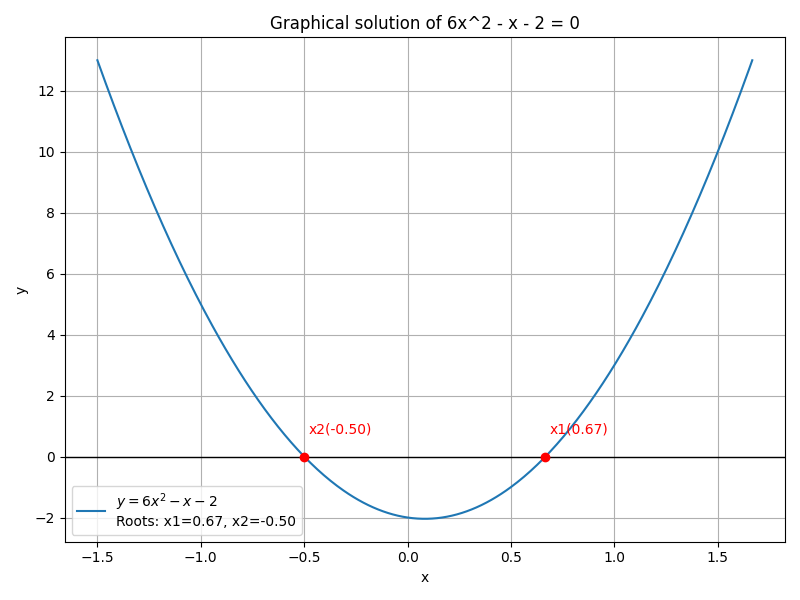
\includegraphics[width=0.8\columnwidth]{../beamer/figs/fig15.png}
    \end{figure}
\end{frame}

\end{document}

